%=====================导=======言==============================
\documentclass[a4paper,11pt]{article}
%======================Include Packages========================

\usepackage[50042]{MCMthesis}  %队号在这里填写
%\usepackage[175,nosheet]{MCMthesis}%这个参数形式可去掉summary sheet首页。
\problem{E}  %选题
%===============设置正文和数学字体=============================
%有些字体需要安装一些字体文件,注意辨别。
%我参照 MCM论文集的字体 使用如下宏包来定制字体。
\usepackage{palatino}
\usepackage{indentfirst}

%设置段落之间的距离,若不需要删除或者注释掉即可。
\setlength\parskip{.5\baselineskip}
\renewcommand{\abstractname}{Summary}
%\def\abstractname{Summary}%可修改摘要名称

%%%%%%%%%%%%%%%%%%%%%%%%%%%%%%%%%%%%%%%%%%%%%%%%%%%%%%%%%%%%%%%%%%%
%%%%%%%%%%%%%%%%%%$$$$$$$==正文开始==$$$$$$$%%%%%%%%%%%%%%%%%%%%%%%
%%%%%%%%%%%%%%%%%%%%%%%%%%%%%%%%%%%%%%%%%%%%%%%%%%%%%%%%%%%%%%%%%%%

%==========================论文标题===============================
\title{Slaking Ukraine's Thirst for Water Based on BP Model}
\author{\small  Team \# 50042 }
\date{\today}
%=================================================================
%==================================================================
\begin{document}
%摘要需要放在maketitle之前才能保证运行正常
%====================摘=======要===================================
\begin{abstract}
To address the water scarcity issue, we firstly establish water carrying capacity coupling model comprising of two sub-models. One is designed for simulation and prediction utilizing 3-level \textbf{BP}(Back Popagation) structure, the other is for comprehensive evaluation by integrating as much information as possible. We choose 13 indexes like \textit{total water resources amount, GDP, population} and so on. In this way the outcome can be transformed into an evaluation result by 5 levels. Then we utilize China's statistics to test our model and it is proved to be feasible for the absolute values of relative error are all within 1\%.

Secondly, we choose Ukraine which was heavily exploited in 2002 to be our target. We use \textbf{PCA}(Principle Component Analysis) and select 8 indexes such as \textit{total withdrawal, GDP, population, wastewater, industrial use, hydroelectricity, agricultural use, municipalities use} to conduct dynamic comprehensive evaluations. SPSS 22 figures out two significant indicators based on data we gathered, namely, \textit{population and industry}. And the ranks of the final score F demonstrate that the overall trend is getting worse; however, situations started to bounce back from 2003 to 2005.

Thirdly, for the sake of minimizing errors, we optimize our model to the new \textbf{TGB} model consisting of triple-inputs, grey model and BP model after we apply Ukraine data into our BP model to complete predictions. The improved TGB model is designed by us and can provide better and more accurate figures. Our prediction results show that Ukraine's water stress issue would continue to deteriorate if no measure was taken.

Next, we propose to establish a desalination plant in southern coastal areas. To select the best cite for this construction, we use \textbf{AHP}(Analysis Hierarchy Process) method and finally choose Odessa considering four important criteria: \textit{geography, local technological level, benefits and profits, and investments}. Apart from all the mentioned work, we also use \textbf{fitting} to simulate a possible clean water curve produced by desalination. In order to quantize its validity, we simply take the quotient of the mean value of annual produced desalination water in 15 years and the mean value of annual total water withdrawal in 15 years, which comes out to be 49.03\%. This figure indicates that our intervention is effective. Last but not least, we evaluate our model in an objective way to help future work.

\begin{keywords}
water stress; Back Propagation; TGB; Grey Prediction; PCA; AHP
\end{keywords}
\end{abstract}

\maketitle

\pagestyle{empty}



\newpage

%==================================================================


%====================生=成=目=录===================================
%\tableofcontents                                                  %
%\newpage
\pagestyle{fancy}                                                 %
%==================================================================

%======================问题介绍====================================
\section{Introduction}

According to the survey conducted by the United Nations, one quarter of the world's population will suffer from water scarcity. Water use has been growing at nearly twice the rate of population over the last century. There's no denying that daily life requires water resources for industrial, agricultural, and residential purposes. Therefore, it is quite necessary and urgent to find out feasible solutions to solve water stress issues.

There are several popular methods to tackle prediction problems. Back Propagation(BP)\cite{1} is an effective method characterized by extensive flexibility self-learning and mapping. It contains knowledge about Artificial Neural Network (ANN) and can approach almost any nonlinear function theoretically and therefore has satisfying results in the field of modeling and prediction of multi-variable nonlinear systems. We utilize this method to directly investigate the internal relationships so as to sheer away from those difficulties that would be met with by other quantization approaches. Hence, Back Propagation lies a solid foundation for researching water resources carrying capacity.

Our group dedicates to establish a model that can both accomplish qualitative and quantitative analysis to give prediction of water stress in 15 years.

\section{Assumptions}

 In order to have a better study on this paper, we simplify our model by the following assumptions:
\begin{itemize}
\item
There will be no droughts, floods, earthquakes and other strong natural disasters in 15 years.
\item
There will be no additional artificial water supply except our determined water strategy intervention in 15 years.
\item
The society will maintain steadily stable and related social policies are kept the same.
\item
Ecological conditions such as weather, climate, hydrology, etc. won't change in 15 years.
\item
Any intervention plan will be effectuated immediately in 2016.
\end{itemize}
Under the above and basic assumptions, we can set out to construct our model (show our approach in detail).

%=============================问题分析==========================================
\section{Establishment of Model}
In order to depict the ability of a region to provide clean water to meet the needs of its population, we adopt an idea of water resources carrying capacity\cite{2}. It is a prevalent idea defined as the ability to support social, economic and environmental development based on predictable level of technology and economy in the context of a certain historical stage. It follows the principle of sustainable development, takes the basic ecological need of water into consideration and requires both reasonable and optimal configurations.

\subsection{Principles of Model}

This model comprises of two sub-models. One sub-model is designed for simulation and prediction. It utilizes 3-level BP structure, where the input vectors are main factors $\Delta X$ while the output vector is water resources carrying capacity $\Delta Y$, and nodes of hidden layers are determined by a specific algorithm. The basic idea is to use known inputs $\Delta X_k$ and outputs $\Delta Y_k$ to train this network so as to meet certain accuracy requirements. The well-trained network would be able to predict future vaules. The other sub-model is for comprehensive evaluation by integrating as much information as possible. In this way the outcome can be transformed into an evaluation result, easy for people to understand\cite{Wengao Lou}.

\subsection{Structure of Model}
(1)\textbf{Overall Structure} The overall model is shown as Figure \ref{overallstructure}.
\begin{figure}[h]
\small
\centering
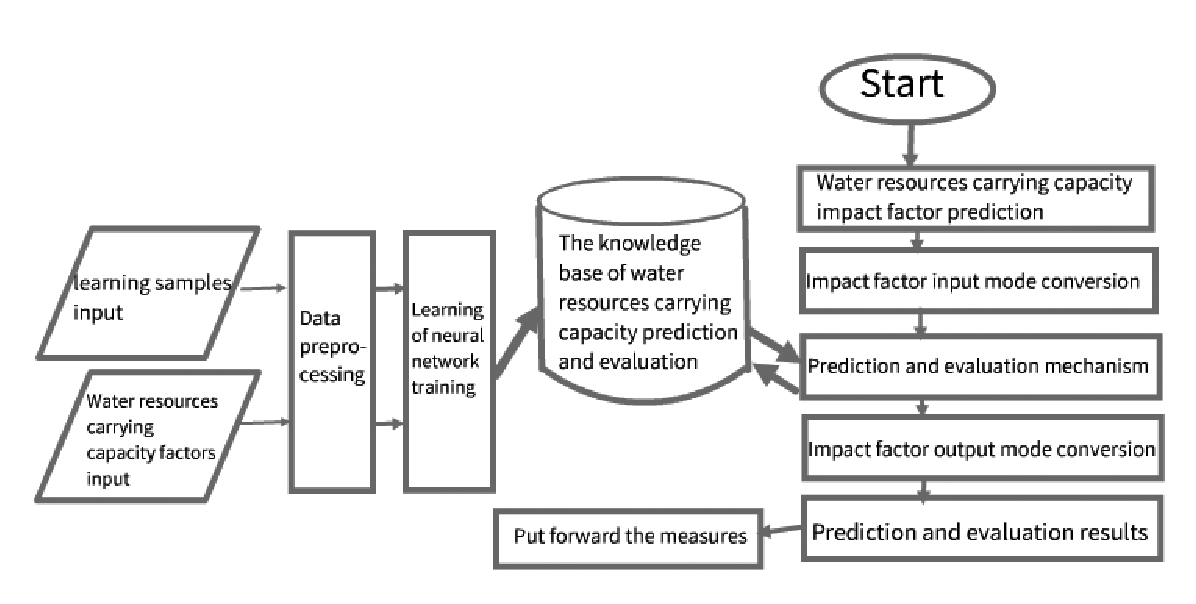
\includegraphics[width=12cm]{./picture/structure.eps}
\caption{Structure of water carrying capacity coupling model based on ANN theory} \label{overallstructure}
\end{figure}

(2)\textbf{Neural Network Structure}
This model consists of the pre-process of data and the main BP network, shown in figure \ref{BP} \cite{Xiangui}. Pre-process section manages data by some rules. BP network differs in layers, outputs, and nodes. We construct a 3-level BP network, namely, input layer, hidden layer, and output layer. The node number m inside this network is determined by the degree of inputs. If the output layer degree is n, then we can get to know the node number in the hidden layer is $L=\dfrac{m\times n}{2}$. The hidden layer output is Sigmoid function.
\begin{figure}[h]
\small
\centering
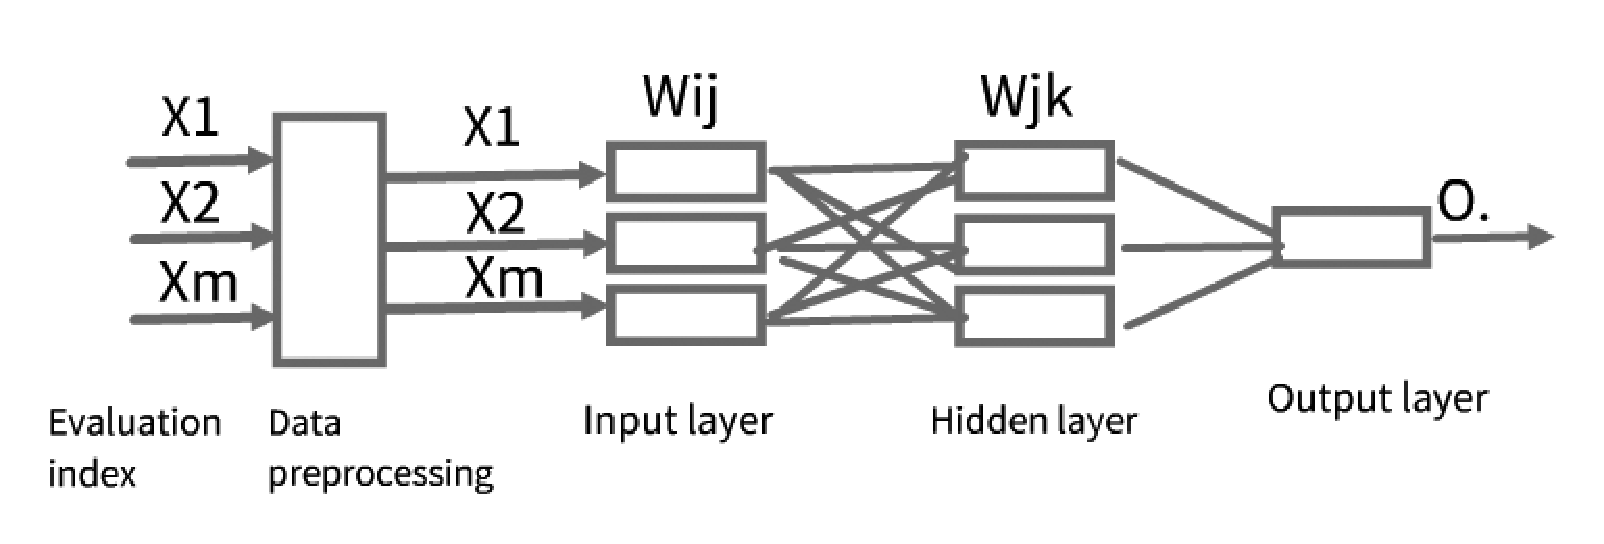
\includegraphics[width=10cm]{./picture/BP.eps}
\caption{ANN topology structure of water carrying capacity model} \label{BP}
\end{figure}

\subsection{Establishment of Evaluation Indicators System}
We need to transform water resources carrying capacity into several specific indicators. Due to the fact that there are numerous factors affecting the prediction and evaluation of carrying capacity and therefore it is essential and critical to distinguish key factors from diverse and complicated causes. Generally speaking, indicators can be sundered into three groups. One group is related with the physical characters such as quality, quantity, etc., another group is about social interventions such as population, economy and policies. The third group is concerning ecological factors such as climates and forests. Considering these three groups, we establish our indicators system shown in figure \ref{System}\cite{Qingwen}.
\begin{figure}[h]
\small
\centering
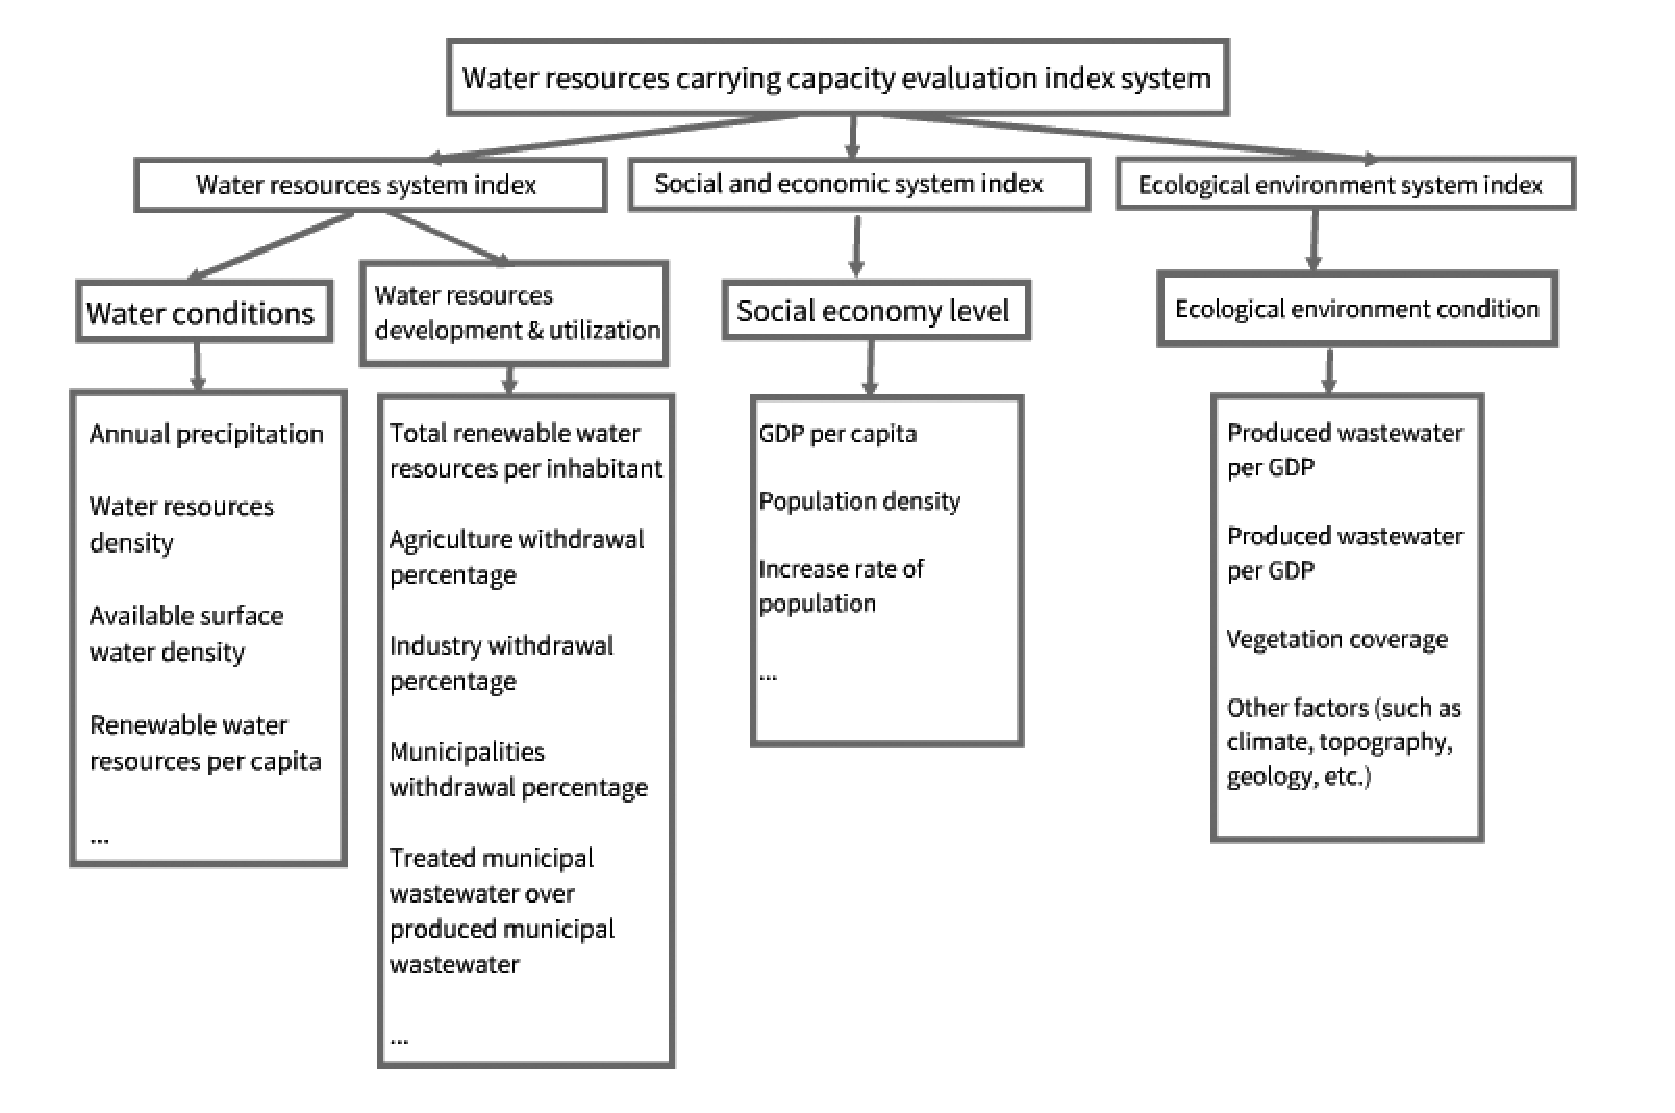
\includegraphics[width=12cm]{./picture/System.eps}
\caption{General evaluation indicators system of water carrying capacity} \label{System}
\end{figure}

On the foundation of this general evaluation indicators system, we can actually use Principal Component Analysis (PCA) to ascertain specific evaluation indicators for a specific region if we know the comprehensive information. Considering the feasibility of modeling in limited time and finite archives that we have found, we select $15$ of all factors that we can think of as the basic indicators. Below is the table of selected evaluation indicators (Table \ref{selected}).
\begin{table} [!htbp]
\centering\caption{Selected indicators of water carrying capacity grade evaluation}
\begin{tabular}{r|l|c}
  \hline
   & anual precipitation & 1 \\
  Quantity of Water & water resources density & 2 \\
   & available surface water density & 3 \\
   & renewable water sources per capita & 4 \\
   \hline
   & renewable water resources per inhabitant & 5 \\
   & agricultural withdrawal percentage&6 \\
  Exploition and Utilization & industrial withdrawal percentage&7 \\
   & municipalities withdrawal percentage &8 \\
   & treated municipal wastewater over  &9 \\
   & produced municipal wastewater & \\
   \hline
   & GDP per capita &10 \\
  Social Econimic Level & population density &11 \\
   & increase rate of population &12 \\
    \hline
   & produced wastewater per GDP &13 \\
  Ecological Environment & produced wastewater per inhabitant &14 \\
   & vegetation coverage &15 \\
  \hline
\end{tabular}\label{selected}
\end{table}
\begin{table} [!htbp]
\centering\caption{Thresholds of water resource carrying capacity evaluation indicators}
\begin{tabular}{|c|c|c|c|c|c|c|c|}
  \hline
  % after \\: \hline or \cline{col1-col2} \cline{col3-col4} ...
  Number & Equation & Level 1 & Level 2 & Level 3 & Level 4 & Level 5 \\
  \hline
  1 & $database$ & $\geq1500$ & $\geq1200$ & $\geq1000$ & $\geq800$ & $<800$ \\
  \hline
  2 & $\dfrac{total\;water\;resource}{territory\;area}$ & $\geq80$ & $\geq60$ & $\geq40$ & $\geq20$ & $<20$ \\
  \hline
  3 & $\dfrac{total\;water\;resource}{territory\;area}$ & $\geq80$ & $\geq60$ & $\geq40$ & $\geq20$ & $<20$ \\
  \hline
  4 & $\dfrac{total\;water\;resource}{population}$ & $\geq5000$ & $\geq4000$ & $\geq3000$ & $\geq2000$ & $<2000$ \\
  \hline
  5 & $\dfrac{total\;water\;withdrawal}{population}$ & $\geq500$ & $\geq450$ & $\geq350$ & $\geq300$ & $<300$ \\
  \hline
  6 & $\dfrac{agricultural\;withdrawal}{total\;withdrawal}$ & $\geq40$ & $\geq30$ & $\geq20$ & $\geq10$ & $<10$ \\
  \hline
  7 & $\dfrac{industrial\;withdrawal}{total\;withdrawal}$ & $\geq40$ & $\geq30$ & $\geq20$ & $\geq10$ & $<10$ \\
  \hline
  8 & $\dfrac{municipalities\;withdrawal}{total\;withdrawal}$ & $\geq40$ & $\geq30$ & $\geq20$ & $\geq10$ & $<10$ \\
  \hline
  9 & $\dfrac{treated\;municipal\;wastewater}{produced\;municipal\;wastewater}$ & $\geq90$ & $\geq70$ & $\geq50$ & $\geq30$ & $<30$ \\
  \hline
  10 & $\dfrac{GDP}{population}$ & $\geq5$ & $\geq3$ & $\geq1$ & $\geq0.6$ & $<0.6$ \\
  \hline
  11 & $\dfrac{population}{territory\;area}$ & $<20$ & $<40$ & $<60$ & $<80$ & $\geq80$ \\
  \hline
  12 & $database$ & $<1\%$ & $\geq1\%$ & $\geq3\%$ & $\geq5\%$ & $\geq7\%$  \\
  \hline
  13 & $\dfrac{produced\;wastewater}{GDP}$ & $\leq10$ & $\leq15$ & $\leq25$ & $\leq30$ & $>30$ \\
  \hline
  14 & $\dfrac{produced\;wastewater}{population}$ & $\leq10$ & $\leq15$ & $\leq25$ & $\leq30$ & $>30$ \\
  \hline
  15 & $\dfrac{vegetation\;area}{territory\;area}$ & $\geq40$ & $\geq30$ & $\geq20$ & $\geq10$ & $<10$ \\
  \hline
  others & $database$ & A & B & C & D & E \\
  \hline
  \end{tabular}\label{criteria}
  \end{table}
After referring to the national water source evaluation criteria as well as research findings we found and considering the status quo, we divide indicators into 5 levels. Threshold values are demonstrated in Table \ref{criteria}.

\section{Validation of Model}
After establishing our model, the next step is to prove its validity. To best test the model, we decide to use available data about China to validate it because we find statistics relating to China more accessible than those of other regions.

\subsection{Introduction about China}
China is a sovereign state in East Asia. It is the world's most populous country, with a population of over 1.35 billion. Covering approximately 9.6 million square kilometers, China is the world's second-largest country by land area, and either the third or fourth-largest by total area, depending on the method of measurement.

There are many rivers and lakes in China, but they mainly belong to the Pacific Ocean water system, which determines the basic trend of the water flow to the East. Precipitation varies greatly across China, the general trend is decreasing from the southeast coast to the northwest inland, southeast coastal areas more than $1600$ mm of precipitation, the Northwest has large areas of annual rainfall in $50$ mm or less.China forest area of over square kilometers, the forest coverage rate is $20.36\%$. China's climate is mainly affected by the monsoon circulation, due to the changing terrain and the formation of a complex climate.

2014 China's GDP per capita was 7595 USD, in 2013 China's GDP per capita was 6264 USD, while in 2012 and 2011 were 6995 USD and 5577 USD, respectively. The proportion of Chinese agriculture accounted for $13.1\%$, the proportion of industry accounted for $46.2\%$, the proportion of service industry rose to $40.7\%$.

\subsection{Application and Validation}
\subsubsection{Data needed in modeling}
According to China's statistical archives since 2000, we have got three important factors to be inputs and select another two factors to be outputs to validate this model. What we do is to use statistics from 2000 to 2011 (12 sets training data) to train the network and use this model to "predict" the conditions in the year of 2012 and 2013. By doing so, we can compare these two sets of outputs with real figures so as to make comments on the model's validity. Table \ref{testi/o} shows the inputs and outputs we selected for China. Meanwhile, Table \ref{testdata} provides details that are needed for validation.
\begin{table}[!htbp]
\centering\caption{Water carrying capacity forecast indicators of BP model}
\begin{tabular}{r|l|c}
  \hline
  % after \\: \hline or \cline{col1-col2} \cline{col3-col4} ...
   & Surface Water Resources&$I_1$\\
  Inputs & Groundwater Resources&$I_2$\\
   & Duplicated Measurement Between Surface Water and Groundwater&$I_3$\\
   \hline
  Outputs & Total Amount of Water Resources&$O_1$\\
   & Water Resources Per Capita&$O_2$\\
  \hline
\end{tabular}\label{testi/o}
\end{table}
\begin{table}[!htbp]
\centering\caption{Statistics used to validate the model}
\begin{tabular}{c|ccc|cc}
  \hline
  % after \\: \hline or \cline{col1-col2} \cline{col3-col4} ...
  Year & $I_1$ & $I_2$ & $I_3$ & $O_1$ & $O_2$ \\
   & $\times10^9 m^3$ & $\times10^9 m^3$ & $\times10^9 m^3$ & $\times10^9 m^3$ & $m^3/person$ \\
   \hline
    2000   &   26561.9   &   8501.9   &   7363.0   &   27700.8   &   2193.9   \\
    2001   &   25933.4   &   8390.1   &   7455.7   &   26867.8   &   2112.5   \\
    2002   &   27243.3   &   8697.2   &   7679.2   &   28261.3   &   2207.2   \\
    2003   &   26250.7   &   8299.3   &   7089.9   &   27460.2   &   2131.3   \\
  2004 & 23126.4 & 7436.3 & 6433.1 & 24129.6 & 1856.3 \\
  2005 & 26982.4 & 8091.1 & 7020.4 & 28053.1 & 2151.8 \\
  2006 & 24358.1 & 7642.9 & 6670.8 & 25330.1 & 1932.1 \\
  2007 & 24242.5 & 7617.2 & 6604.5 & 25255.2 & 1916.3 \\
  2008 & 26377.0 & 8122.0 & 7064.7 & 27434.3 & 2071.1 \\
  2009 & 23125.2 & 7267.0 & 6212.1 & 24180.2 & 1816.2 \\
  2010 & 29797.6 & 8417.0 & 7308.2 & 30906.4 & 2310.4 \\
  2011 & 22213.6 & 7214.5 & 6171.4 & 23256.7 & 1730.2 \\
  \hline
  2012 & 28371.4 & 8416.1 & 7260.6 & 29526.9 & 2186.1 \\
  2013 & 26839.5 & 8081.1 & 6962.7 & 27957.9 & 2059.7 \\
  \hline
\end{tabular}
\label{testdata}
\end{table}

\subsubsection{Results}
After training the network using 12 set data, we get the predicted values. Below demonstrates the comparison between estimated values and real values (Table \ref{testresults}, Appendix A). To see the whole process clearly and vividly, we use Matlab 2015a to plot two curves to show the results. The figure is shown in Figure \ref{testresultfigure}(Appendix B).
\begin{figure}[!htbp]
\small
\centering
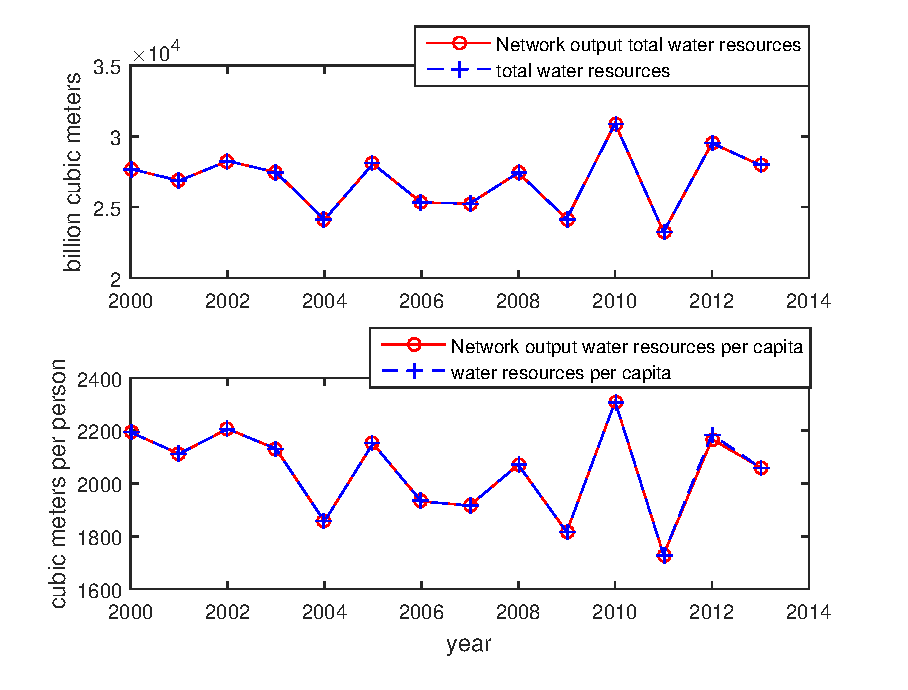
\includegraphics[width=9cm]{./picture/testresults.eps}
\caption{Plot of testing results of BP model} \label{testresultfigure}
\end{figure}
\begin{table}[!htbp]
\centering\caption{Testing Result of BP model}
\begin{tabular}{c|ccc}
  \hline
  % after \\: \hline or \cline{col1-col2} \cline{col3-col4} ...
  Year &  & 2012 & \\
  \hline
  & Real Values & Estimated Values & Absolute Value of Relative Error/\%   \\
  \hline
  $O_1$ & 29526.9 & 29518.0 & 0.03\% \\
  $O_2$ & 2186.1  & 2168.0  & 0.8\% \\
  \hline
  Year &  & 2013 & \\
  \hline
  & Real Values & Estimated Values & Absolute Value of Relative Error/\% \\
  \hline
  $O_1$ & 27957.9 & 27966.0 & 0.03\% \\
  $O_2$ & 2059.7  & 2061.0  & 0.6\% \\
  \hline
\end{tabular}\label{testresults}
\end{table}

We can easily see that the relative errors are all smaller than $1\%$, which indicates a good prediction and the validity of our model. Through this validation test, our model is proved to be effective and accurate to tackle water resources carrying capacity.
\section{Investigation}
By looking through the UN water scarcity map, we finally chose Ukraine whose water resources are heavily exploited (Figure \ref{world}).
\begin{figure}[!htbp]
\small
\centering
\includegraphics[width=12cm]{./picture/world.eps}
\caption{Water stress indicator in major basins (Ukraine zoomed in)} \label{world}
\end{figure}
\subsection{Water Resources in Ukraine}
The country can be divided into seven major river basins, all of them discharging into the Black Sea except the Western Bug which flows towards the Baltic Sea:
\begin{itemize}
\item \textbf{The Dnipro (called Dnieper in Belarus) basin:}
covering about 65 percent of the country. The Dnipro river rises in the Russian Federation, then flows into Belarus before entering Ukraine. Its main affluents in Ukraine are: the Desna river (on the left bank) and the Pripyat river (on its right bank).
\item \textbf{The Dniester (called Nistru in the Republic of Moldova) basin:}
covering 12 percent of the country. It flows into the Republic of Moldova before re-entering Ukraine some 50 km before its mouth in the Black Sea.
\item \textbf{The Danube basin:}
covering 7 percent of the country. The Danube is the river with the largest number of riparian countries in the world. Some affluents of the Danube rise in Ukraine in the Carpathian mountains, flow into neighbouring countries, and then join the mainstream of the Danube before its mouth in the Black Sea.
\item \textbf{The coastal basin:}
covering 7 percent of the country. It groups all the small rivers that flow directly into the Sea of Azov and the Black Sea, including all the Crimean rivers.
\item \textbf{The Donets basin:}
covering 4 percent of the country. It rises in the Russian Federation, and flows through Ukraine for about 450 km in its eastern part before re-entering the Russian Federation.
\item \textbf{The Southern Bug (Pivdennyi Buh in Ukrainian) basin:}
covering 3 percent of the country. It is an internal river basin.
\item \textbf{The Western Bug (Zakhidnyi Buh in Ukrainian) and San basins:}
covering 2 percent of the country. The Western Bug river rises in Ukraine, flows to the north, forming the border with Poland and then the border between Poland and Belarus, and finally flows into the Narew river in Poland, a tributary of the Vistula river.
\end{itemize}

IRSWR are estimated at 50100 million $m^3$/year (Figure \ref{table1}) and incoming RSWR at 120180 million $m^3$. Therefore, the total RSWR are estimated at 170280 million $m^3$/year.

\begin{figure}[!htbp]
\small
\centering
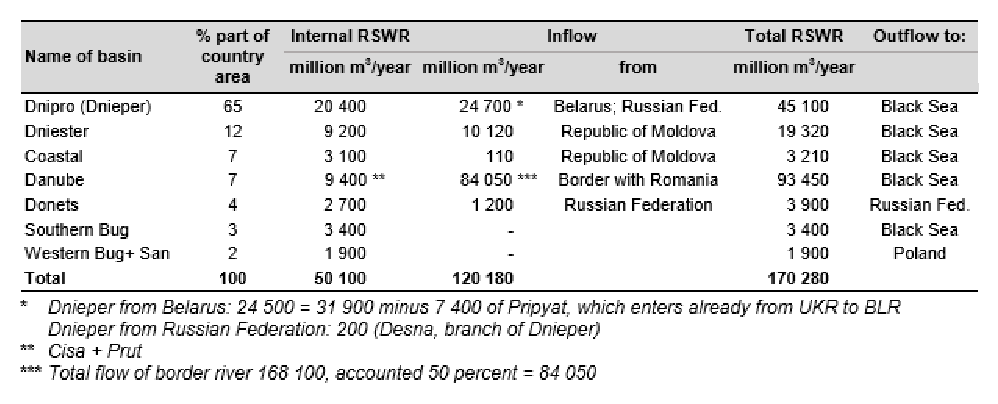
\includegraphics[width=12cm]{./picture/Table1.eps}
\caption{Ukraine renewable surface water sources by major river basin} \label{table1}
\end{figure}

\begin{figure}[!htbp]
\small
\centering
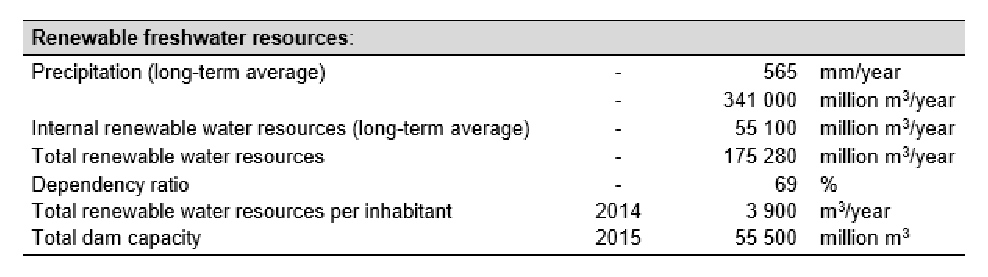
\includegraphics[width=12cm]{./picture/Table2.eps}
\caption{Ukraine renewable water sources} \label{table2}
\end{figure}

Internal renewable groundwater resources are estimated at 22000 million $m^3$/year. Artesian wells are found at an average depth of 100-150 m in the north of the country and at 500-600 m in the south. The overlap between surface and groundwater resources has been estimated at 17000 million $m^3$/year, which brings the total renewable water resources to 175280 million $m^3$ (170280+22000-17000) (Figure \ref{table2}).

\subsection{Water Use in Ukraine}

Water use details are shown in Table \ref{wateruse} \cite{Liyu Han}.
\begin{table}[h]
\centering\caption{Ukraine water use in 1998-2005 (unit:$\times 10^8 m^3$)}
\begin{tabular}{c|c|c|c|c|c|c|c|c}
  \hline
  % after \\: \hline or \cline{col1-col2} \cline{col3-col4} ...
  Year & 1998 & 1999 & 2000 & 2001 & 2002 & 2003 & 2004 & 2005 \\
  \hline
  Total Withdrawal & 190.27 & 197.48 & 182.82 & 175.77 & 162.99 & 150.39 & 146.94 & 150.83 \\
  \hline
  Total comsumption & 139.35 & 144.68 & 132.22 & 124.82 & 119.01 & 114.03 & 98.27 & 98.74 \\
  \hline
  Municipalities & 34.81 & 34.59 & 33.00 & 34.21 & 33.50 & 32.50 & 30.82 & 30.36 \\
  Industrial & 76.52 & 71.00 & 67.26 & 64.89 & 60.54 & 55.28 & 51.07 & 51.27 \\
  Agricultural & 37.02 & 39.09 & 31.96 & 25.77 & 24.97 & 26.25 & 16.38 & 17.11 \\
  \hline
\end{tabular}\label{wateruse}
\end{table}

\subsection{Causes of Water Scarcity}
\subsubsection{Modeling to find key factors}
Based on the data that we gathered about Ukraine, we found 8 different types of statistics. To better understand the internal relationships amongst these figures, we apply Principal Component Analysis (PCA)\cite{Lang Xu} to conduct dynamic comprehensive evaluations. Suppose $X_1$:Total withdrawal, $X_2$:GDP, $X_3$:Population, $X_4$:Wastewater, $X_5$:Industrial use, $X_6$:Hydroelectricity, $X_7$:Agricultural use, $X_8$:Municipalities use. Data are shown in Table \ref{Ukrainedata}.
\begin{table}[h]
\centering\caption{Statistics of water resources and economy of Ukraine}
\begin{tabular}{c|cccccccc}
  \hline
  % after \\: \hline or \cline{col1-col2} \cline{col3-col4} ...
  Year & $X_1$ & $X_2$ & $X_3$ & $X_4$ & $X_5$ & $X_6$ & $X_7$ & $X_8$ \\
   & $\times 10^8 m^3$ & $\times 10^8 USD$ & $\times 10^6$ & $\times 10^8 m^3$ & \% & \% & $\times 10^8 m^3$ & $\times 10^8 m^3$ \\
   \hline
  1998 & 190.27 & 418.83 & 50.28 & 50.92 & 54.91 & 9.3 & 37.02 & 34.81  \\
  1999 & 197.48 & 315.81 & 49.89 & 52.80 & 49.07 & 8.7 & 39.09 & 34.59  \\
  2000 & 182.82 & 312.62 & 49.47 & 52.60 & 50.87 & 6.4 & 31.96 & 33.00  \\
  2001 & 175.77 & 380.09 & 48.67 & 50.95 & 51.99 & 6.9 & 25.77 & 34.21  \\
  2002 & 162.99 & 423.93 & 48.23 & 43.98 & 50.87 & 5.6 & 24.97 & 33.50  \\
  2003 & 150.39 & 501.33 & 47.79 & 36.36 & 48.48 & 5.0 & 26.25 & 32.50  \\
  2004 & 146.94 & 648.81 & 47.46 & 48.67 & 51.97 & 6.6 & 16.38 & 30.82  \\
  2005 & 150.83 & 828.81 & 47.09 & 52.09 & 51.92 & 6.5 & 17.11 & 30.36  \\
  \hline
\end{tabular}\label{Ukrainedata}
\end{table}

After using SPSS 22 to process the data, we get correlation coefficients matrix of driving force factors (Table \ref{correlation}). We can conclude from Table \ref{correlation} that selected factors are correlated, which is the vital basis to continue using PCA.
\begin{table}[h]
\centering\caption{Correlation coefficients matrix of driving force factors}
\begin{tabular}{c|cccccccc}
  \hline
   & $X_1$ & $X_2$ & $X_3$ & $X_4$ & $X_5$ & $X_6$ & $X_7$ & $X_8$ \\
  \hline
  $X_1$ & 1 &  &  &  &  &  &  &  \\
  $X_1$ & -0.779 & 1 &  &  &  &  &  &  \\
  $X_1$ & 0.961 & -0.809 & 1 &  &  &  &  &  \\
  $X_1$ & 0.550 & -0.072 & 0.411 & 1 &  &  &  &  \\
  $X_1$ & 0.764 & -0.285 & 0.745 & 0.671 & 1 &  &  &  \\
  $X_1$ & 0.922 & -0.811 & 0.950 & 0.223 & 0.643 & 1 &  &  \\
  $X_1$ & 0.849 & -0.874 & 0.867 & 0.122 & 0.542 & 0.868 & 1 &  \\
  $X_1$ & 0.957 & -0.789 & 0.985 & 0.403 & 0.745 & 0.930 & 0.908 & 1 \\
  \hline
\end{tabular}\label{correlation}
\end{table}

Table \ref{eigenvalues} shows that first two dominant components have contributed 92.766\%. Therefore, these two components can effectively reflect the water resources carrying capacity. Besides, from component matrix in Table \ref{copomentmatrix}, we know that the first dominant component is positively related to $X_1$, $X_3$, $X_4$, $X_5$, $X_6$, $X_7$, $X_8$ while it is negatively related to $X_2$. To recap, industry and population are major factors.
\begin{table}[h]
\centering\caption{Eigen values and squared loading of the principal components}
\begin{tabular}{c|c|c|c}
  \hline
  % after \\: \hline or \cline{col1-col2} \cline{col3-col4} ...
  Component & Total & \% of Variance & Cumulative \% \\
  \hline
  1 & 6.072 & 75.900 & 75.900 \\
   \hline
  2 & 1.349 & 16.866 & 92.766 \\
  \hline
\end{tabular}\label{eigenvalues}
\end{table}
\begin{table}[h]
\centering\caption{Component matrix}
\begin{tabular}{c|cccccccc}
  \hline
  % after \\: \hline or \cline{col1-col2} \cline{col3-col4} ...
  Component & $X_1$ & $X_2$ & $X_3$ & $X_4$ & $X_5$ & $X_6$ & $X_7$ & $X_8$ \\
  \hline
  1 & 0.984 & -0.818 & 0.988 & 0.441 & 0.759 & 0.946 & 0.905 & 0.987 \\
  2 & 0.102 & 0.466 & -0.014 & 0.833 & 0.539 & -0.180 & -0.323 & -0.020 \\
  \hline
\end{tabular}\label{copomentmatrix}
\end{table}

Table \ref{scores} shows that $F_1$ and $F_2$ are scores of dominant component, F refers to the final score. The higher the scores is, the better the water resources carrying capacity will be, and vice versa. The ranks demonstrate that the overall trend is getting worse; however, from 2003 to 2005, situations started to bounce back.
\begin{table}[h]
\centering\caption{Scores of water resources carrying capacity in 1998-2005}
\begin{tabular}{c|ccc|c}
  \hline
  % after \\: \hline or \cline{col1-col2} \cline{col3-col4} ...
  Year & $F_1$ & $F_2$ & F & Rank \\
   \hline
  1998 & 1.27993& 0.43103& 1.044164& 1\\
  1999 & 1.25846& 0.30825& 1.007161& 2\\
  2000 & 0.54080& -0.5651& 0.315157& 3\\
  2001 & 0.29376& -0.5776& 0.125546& 4\\
  2002& -0.26058& -1.00844& -0.36786& 5\\
  2003& -0.78978& -1.76171& -0.89657& 8\\
  2004& -1.08912& 0.69091& -0.71011& 7 \\
  2005& -1.23347& 1.45422& -0.69093& 6 \\
  \hline
\end{tabular}\label{scores}
\end{table}

After analysing available data, we draw a conclusion that Ukraine mainly suffers from physical scarcity rather than economic scarcity.
\subsubsection{Causes}
Reasons for \textbf{physical scarcity} mainly contains the following environmental drivers:
\begin{itemize}
\item water resources per capita shortage
\item water dependence
\item uneven temporal and spatial distribution of water resources
\end{itemize}

In 2005, water resources per capita in Ukraine is about 1100 $m^3$ and less than 1700 $m^3$, which is the international water shortage warning line standard. Another fact that needs special attention is that the European average figure is 9089 $m^3$, way higher than Ukraine. Therefore, this bare fact implies that Ukraine belongs to water shortage countries.

What's more, from Figure \ref{table2} we notice a significant value, that is "Dependency ratio". Ukraine's dependency ratio is 69\%. This figure illustrates to what extent this country relies on water inflows from contiguous countries. This indicates that Ukraine suffers from water dependence, which can also answer to the water stress issue.

Besides, temporal and spatial distribution of water resources in Ukraine is quite uneven. Generally speaking, water resources are abundant in the north and northwest while water resources are scarce in the south. Additionally, water mainly flows in spring, accounting for roughly 60\% and 90\% of the annual water resources in northern and southern areas respectively.

As for economic scarcity, based on the statistics, people in Ukraine have convenient access to clean water (access intex is 96\% for total population, shown in Figure \ref{plot11}).Hence, we speculate that the infrastructure to provide water in Ukraine is, comparatively, comprehensively constructed.

\begin{figure}[hp]
\small
\centering
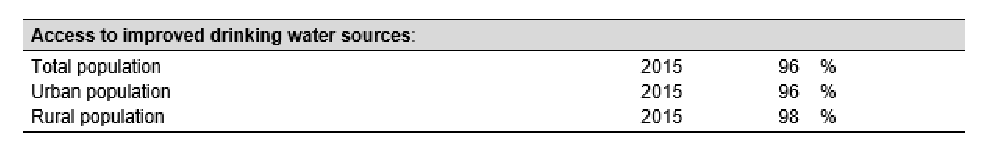
\includegraphics[width=12cm]{./picture/plot11.eps}
\caption{Access of water in Ukraine in 2010} \label{plot11}
\end{figure}

Reasons for \textbf{social factors} mainly contains the following drivers:
\begin{itemize}
\item excessive consumption per capita
\item water-consuming industrial structure
\end{itemize}

According to the results that we have found, the daily water consumption per capita in Ukraine is as high as 320 liters while the average level in western Europe is 100-200 liters. Figures are even higher in busy cities like Odessa and Kiev. This value shows that inhabitants in Ukraine use water extravagantly and lack of water saving consciousness.

Additionally, results produced by PCA conspicuously show that industrial withdrawal is always the dominant consumers (shown in Figure \ref{plot})and it has similar trend with total withdrawal curve. Hence, we can conclude that industrial withdrawal affects total withdrawal the most. When we compare this ratio with other countries, we find that Ukraine's percentage is relatively bigger, indicating the many industries in Ukraine is water-consuming.

\begin{figure}[hp]
\small
\centering
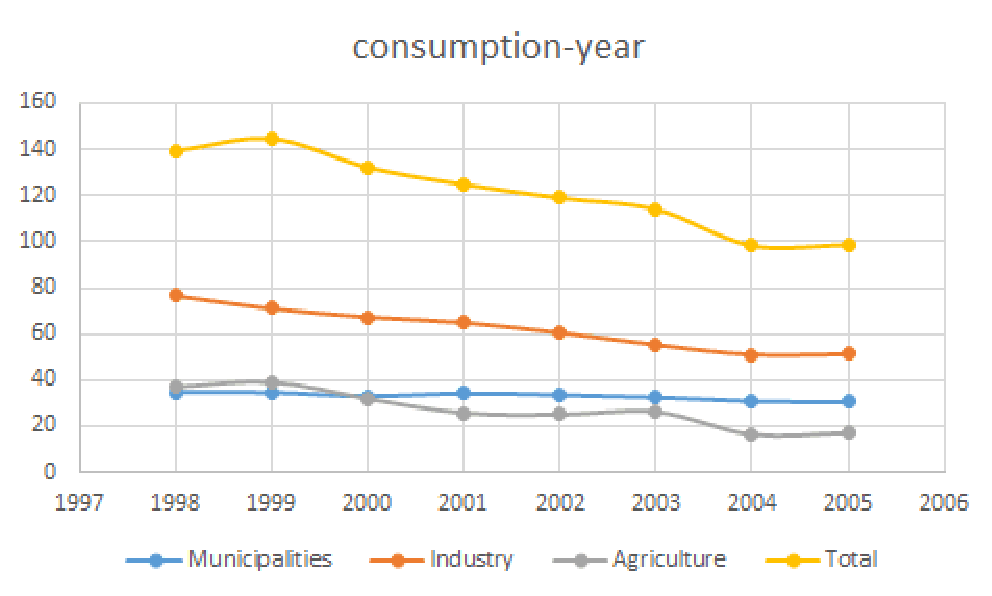
\includegraphics[width=9cm]{./picture/plot.eps}
\caption{Ukraine water consumption in 1998-2005} \label{plot}
\end{figure}

\section{Model Application to Ukraine}
By using data that we have found plus the model that we have established, we get the predicted values for the following 15 years. Table \ref{predicted1} demonstrates the overall figures.
\begin{table}[!htbp]
\centering\caption{Predicted total water withdrawal in Ukraine in 1998-2030 using BP model}
\begin{tabular}{c|c|c|c|c|c|c|c|c|c}
  \hline
  % after \\: \hline or \cline{col1-col2} \cline{col3-col4} ...
  Year & 1998 & 1999 & 2000 & 2001 & 2002 & 2003 & 2004 & 2005 & 2006 \\
  Value & 190.256& 197.342& 182.939& 175.709& 161.469& 149.526& 146.948& 150.797& 151.391\\
  \hline
  Year & 2007 & 2008 & 2009 & 2010 & 2011 & 2012 & 2013 & 2014 & 2015 \\
  Value & 151.506& 151.549& 151.578& 151.599& 151.615& 151.627& 151.635& 151.639& 151.64\\
  \hline
  Year & 2016 & 2017 & 2018 & 2019 & 2020 & 2021 & 2022 & 2023 & 2024 \\
  Value & 151.638& 151.633& 151.626& 151.616& 151.603& 151.589& 151.571& 151.552& 151.53\\
  \hline
  Year & 2025 & 2026 & 2027 & 2028 & 2029 & 2030 & & &  \\
  Value & 151.506& 151.479& 151.45& 151.418& 151.385& 151.348 &&&\\
  \hline
\end{tabular}\label{predicted1}
\end{table}

However, when we compare predicted values in 1998-2005 with real values, we calculated residual $\delta$ and found that the absolute value of residual $|\delta|=0.3128$ (Appendix C), which is a little large. It indicates that the current model may be not precise enough to predict the future conditions when doing long-term estimation. Hence, we have to optimize our model to ensure its reliability.

\subsection{Optimization of Model}
\subsubsection{Introduction of improved model}

This improved model can be represented by TGB (Triple-inputs Grey Back Propagation model).
\begin{itemize}
\item \textbf{T}:triple-inputs. Three inputs are derived from GM(1,1), DGM(2,1), and Grey Verhulst model\cite{Jianyong Liu} accordingly. They are used as inputs of BP model. GM(1,1) refers to Grey Forcasting Model, and (1,1) represents first order differential equations with sole variable. Similarly, DGM(2,1) refers to Discrete Grey Forecasting  Model. and Grey Verhulst Model is designed to describe the process to approach final values.
\item \textbf{G}:grey model. Grey prediction conducts association analysis by system identifying the similarity of system factors to generate the law of the system change. By generating data sequence of strong regularity, one can establish the corresponding differential equation model, to predict the trend.
\item \textbf{B}:BP model.This is exactly what we have established before improvement.
\end{itemize}

The structure of this new TGB model\cite{Shitang Ke} can be represented by Figure \ref{TGB}.
\begin{figure}[hp]
\small
\centering
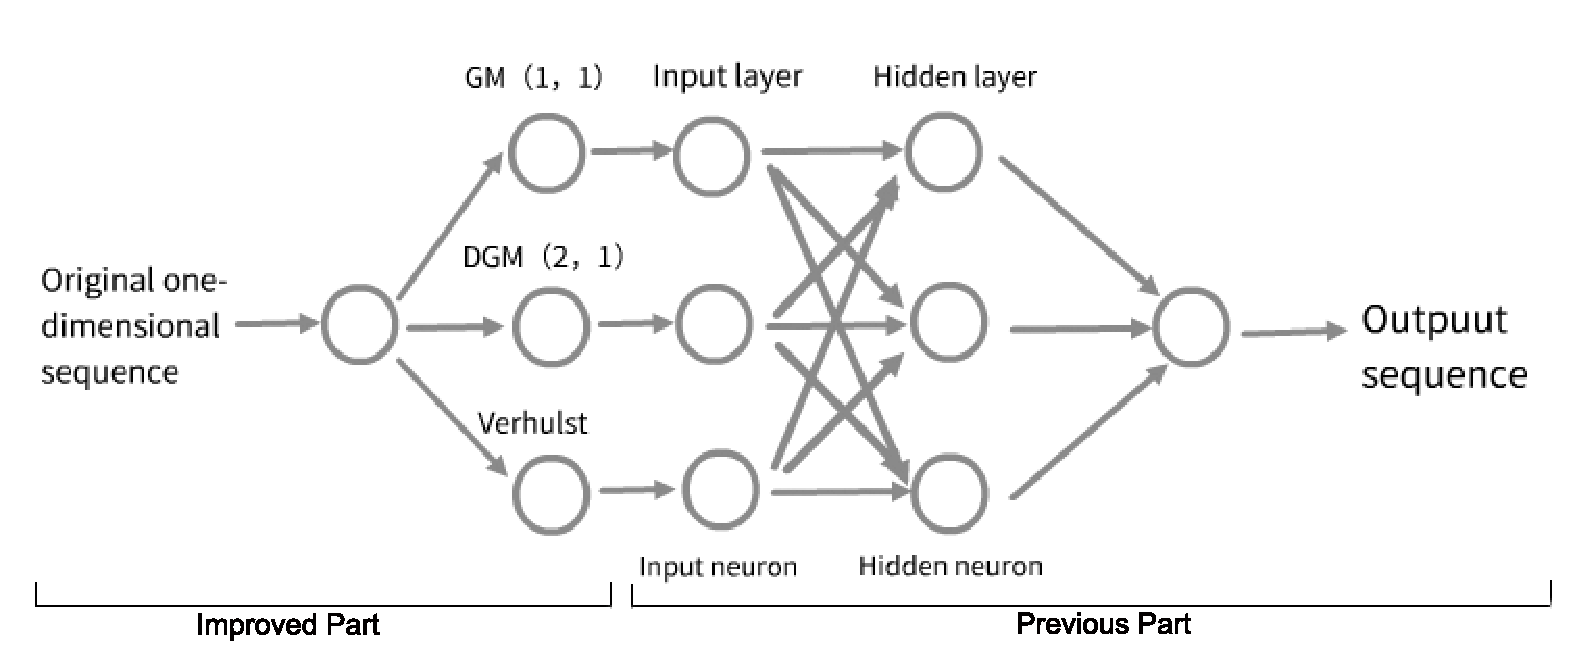
\includegraphics[width=14cm]{./picture/TGB.eps}
\caption{Structure of TGB model} \label{TGB}
\end{figure}

\subsubsection{Establishment of TGB Model}

Let $m$ be the original sequence length, $n$ be the predicted sequence length.\\
\textbf{Step 1:} Use GM(1,1) (Appendix D), DGM (Appendix E), and Verhulst (Appendix F) model to figure out $m$ simulation values and $n$ predicted values.\\
\textbf{Step 2:} Utilize $m$ simulation values to train the network until the precision meets the standard (Appendix G).\\
\textbf{Step 3:} Apply $n$ predicted values to be inputs into the network, and the outputs are what TGB model finds out.

Three models have their own advantages with respect to different types of data. Table \ref{comparison} (Appendix H) shows the advantage of TGB model compared to a single GM(1,1), DGM and Verhulst model. We can clearly see that TGB model has the smallest absolute of residual and therefore, has the best prediction.
\begin{table}[!htbp]
\centering\caption{Comparison of 4 models}
\begin{tabular}{c|c|c}
  \hline
  % after \\: \hline or \cline{col1-col2} \cline{col3-col4} ...
  Model & Absolute Value of Residual$|\delta|$ & Relative Error \\
  \hline
  GM(1,1) & 0.0271 & 0.1606 \\
  DGM(2,1) & 0.0071 & 1.25$\times 10^{-5}$ \\
  Verhulst & 0.0115 & 5.0$\times 10^{-5}$ \\
  TGB & 0.0039 & 2.39$\times 10^{-5}$ \\
  \hline
\end{tabular}\label{comparison}
\end{table}

\subsection{Prediction results}

Applying the new TGB model, we get the following outputs. Figure \ref{TGBresults} (a)(b)(c)demonstrates 3 processed inputs using GM(1,1), DGM(2,1) and Verhulst. Figure \ref{TGBresults} (d) shows the training results of TGB model, and Figure \ref{curve} (Appendix I)shows the final predicted value of total water withdrawals. Detailed values are in Table \ref{predicted2} (Appendix 9).
\begin{figure}[!htbp]
\small
\centering
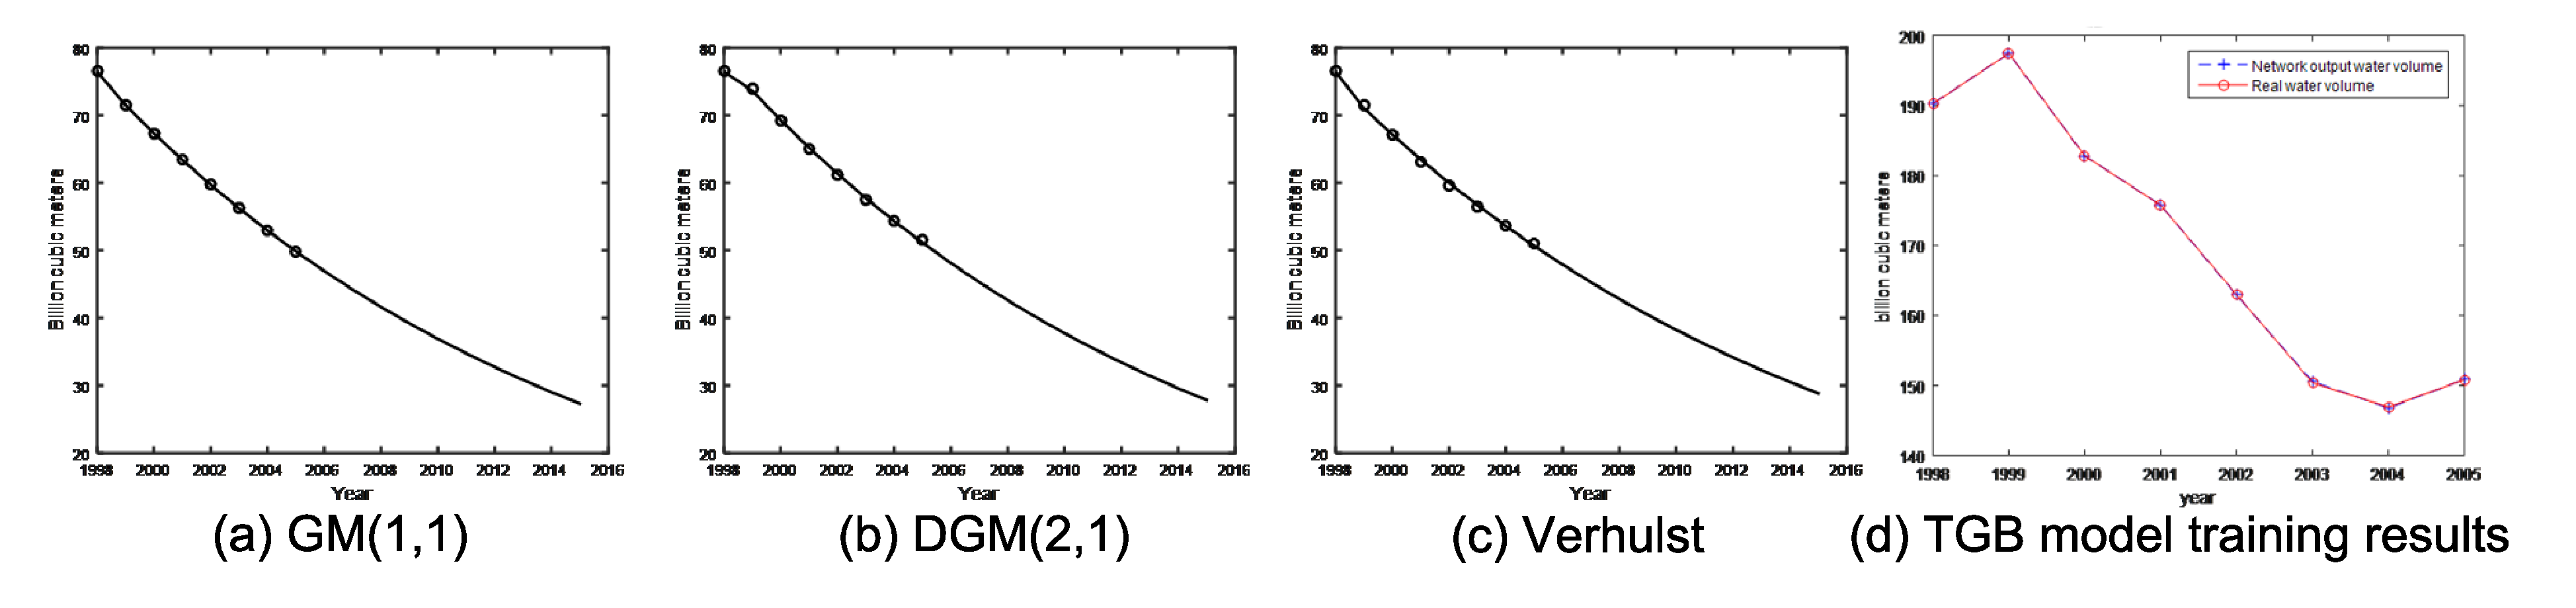
\includegraphics[width=14cm]{./picture/TGBresults.eps}
\caption{TGB model results} \label{TGBresults}
\end{figure}
\begin{figure}[!htbp]
\small
\centering
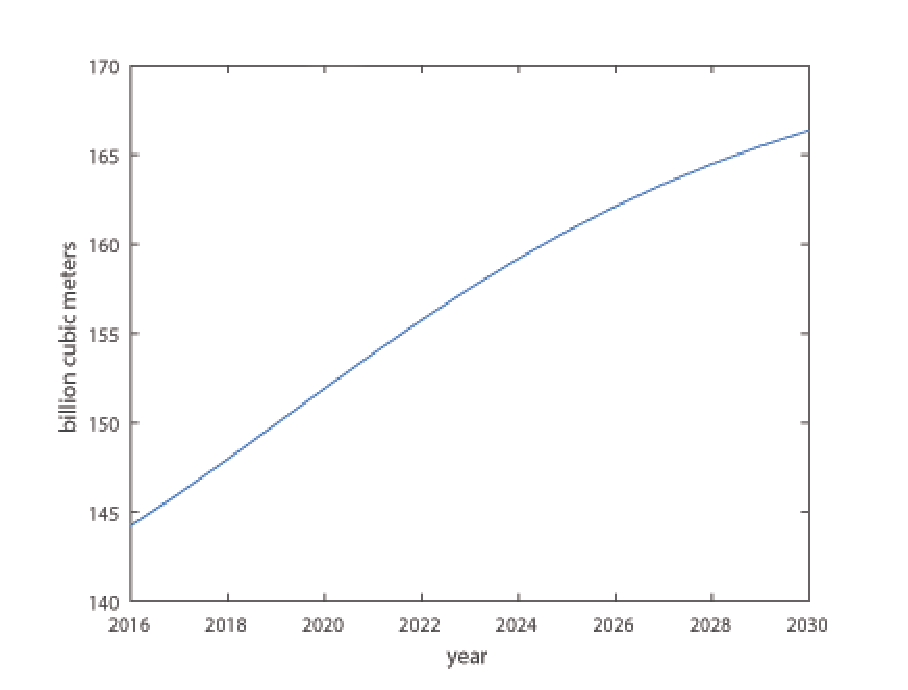
\includegraphics[width=8cm]{./picture/curve.eps}
\caption{Ukraine predicted water withdrawal in 2016-2030} \label{curve}
\end{figure}
\begin{table}[!htbp]
\centering\caption{Predicted total water withdrawal in Ukraine in 1998-2030 using TGB model}
\begin{tabular}{c|c|c|c|c|c|c|c|c|c}
  \hline
  % after \\: \hline or \cline{col1-col2} \cline{col3-col4} ...
  Year & 1998 & 1999 & 2000 & 2001 & 2002 & 2003 & 2004 & 2005 & 2006 \\
  Value & 190.272& 197.482& 182.822& 175.777& 162.994& 150.395& 146.945& 150.834& 149.925\\
  \hline
  Year & 2007 & 2008 & 2009 & 2010 & 2011 & 2012 & 2013 & 2014 & 2015 \\
  Value & 149.049& 148.963& 148.364& 147.946& 147.34& 146.55& 145.079& 144.309& 144.162\\
  \hline
  Year & 2016 & 2017 & 2018 & 2019 & 2020 & 2021 & 2022 & 2023 & 2024 \\
  Value & 144.232& 146.041& 147.957& 149.93& 151.913& 153.862& 155.74& 157.52& 159.181\\
  \hline
  Year & 2025 & 2026 & 2027 & 2028 & 2029 & 2030 & & &  \\
  Value & 160.71& 162.103& 163.359& 164.484& 165.484& 166.369 &&&\\
  \hline
\end{tabular}\label{predicted2}
\end{table}

\subsection{Analysis of Prediction}
Our prediction results of total withdrawal is basically monotonic and will increase with time passing by. However, this figure seems to remain steady from the year of 2030. In other words, water stress in Ukraine is going to deteriorate, which seems to be an identical result with World Resource Institute(WRI)\cite{wri}. Figure \ref{demand} and Figure \ref{waterstress} shows the projected water demand and overall water stress in Ukraine conducted by WRI. Hence, Ukraine government has to intervene this water stress issue before it is too late.
\begin{figure}[hp]
\small
\centering
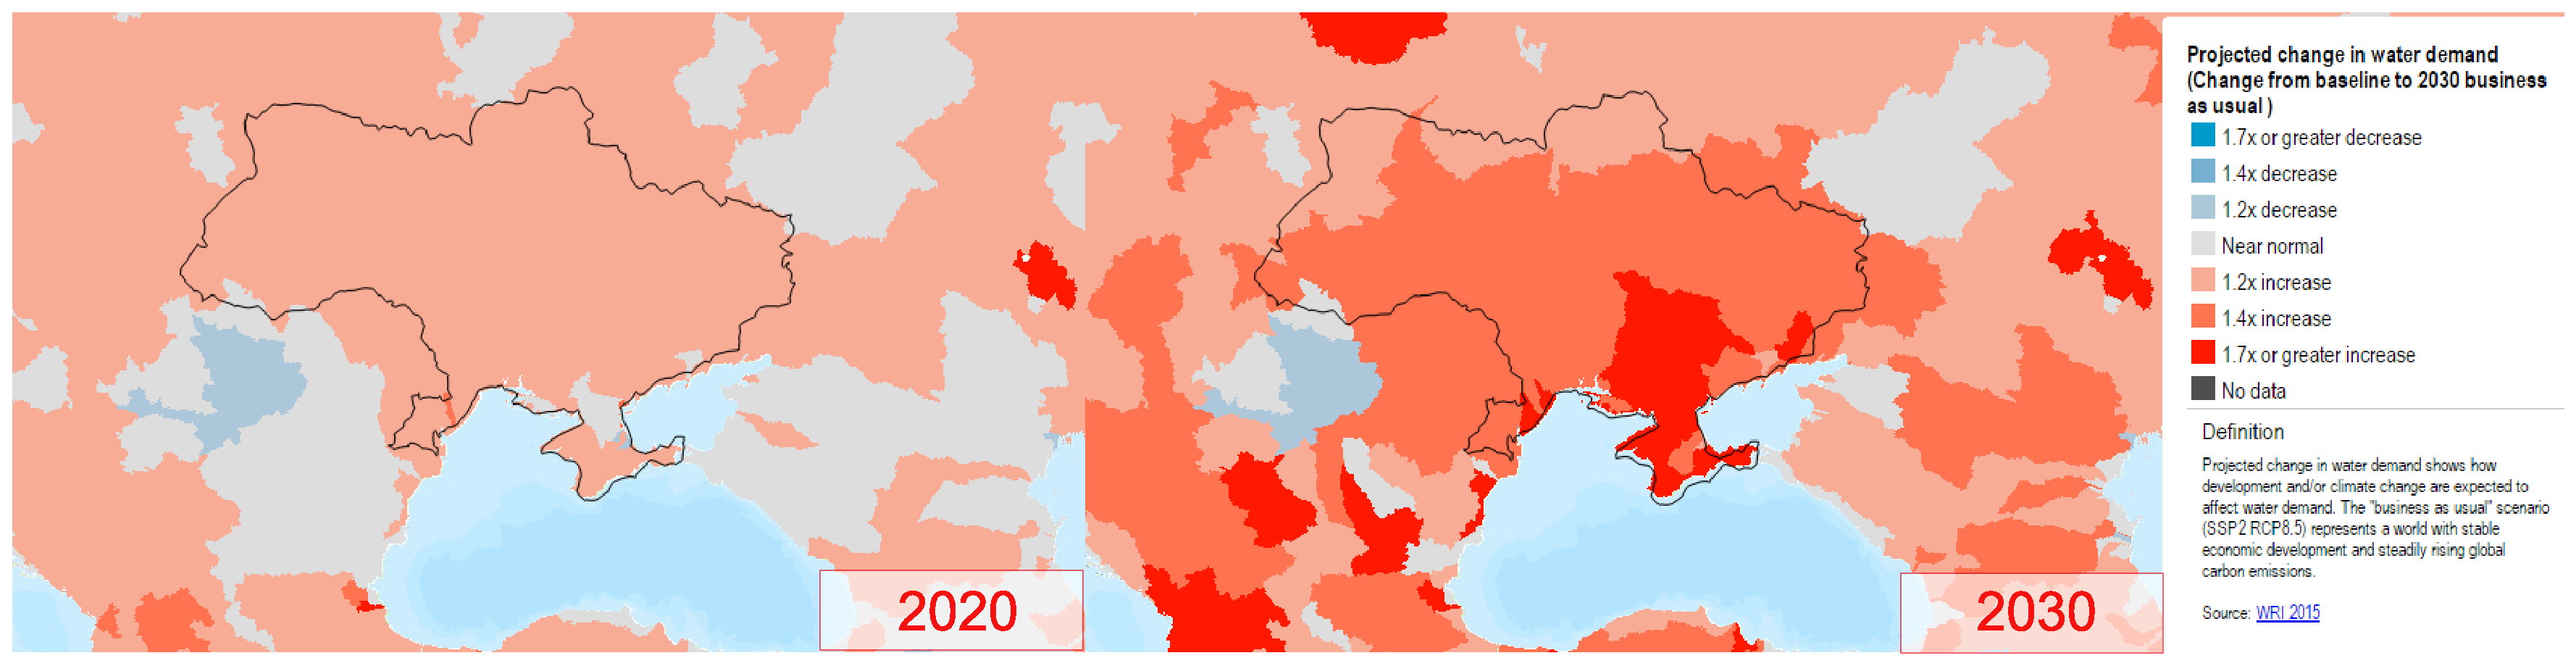
\includegraphics[width=14cm]{./picture/demand.eps}
\caption{Ukraine projected change in water demand (WRI)} \label{demand}
\end{figure}
\begin{figure}[hp]
\small
\centering
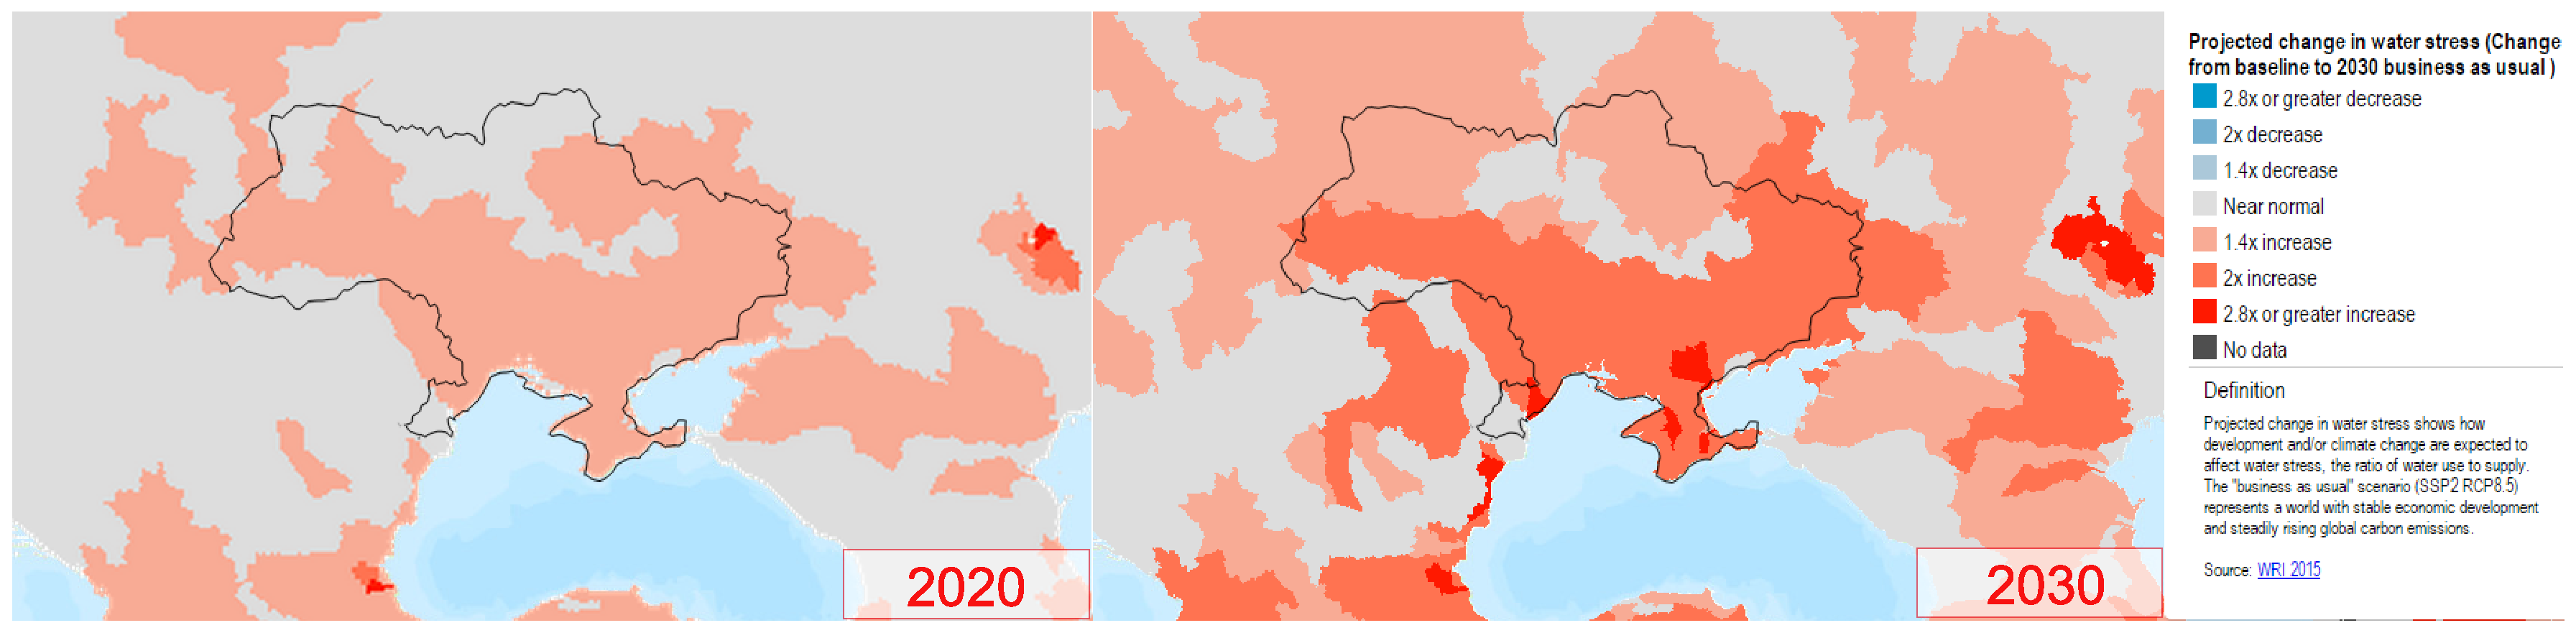
\includegraphics[width=14cm]{./picture/yuce.eps}
\caption{Ukraine projected change in water stress (WRI)} \label{waterstress}
\end{figure}

\section{Intervention plan}
There are some feasible approaches to tackle the water stress that would occur in Ukraine. Based on the fact that Ukraine is a coastal country and southern places suffer more from water stress, construction of desalination plants is an ideal approach. In recent years people have already acquired many novel and innovative methods to implement desalination, therefore this method is ensured by technology.
\subsection{AHP modeling}
By searching for geological information combined with our analysis, we select 4 potential locations to construct a desalination: Odessa, Kherson, Simferopol, and Berdyansk. These four places are marked in red dots in the following figure \ref{location}.
\begin{figure}[!htbp]
  \centering
  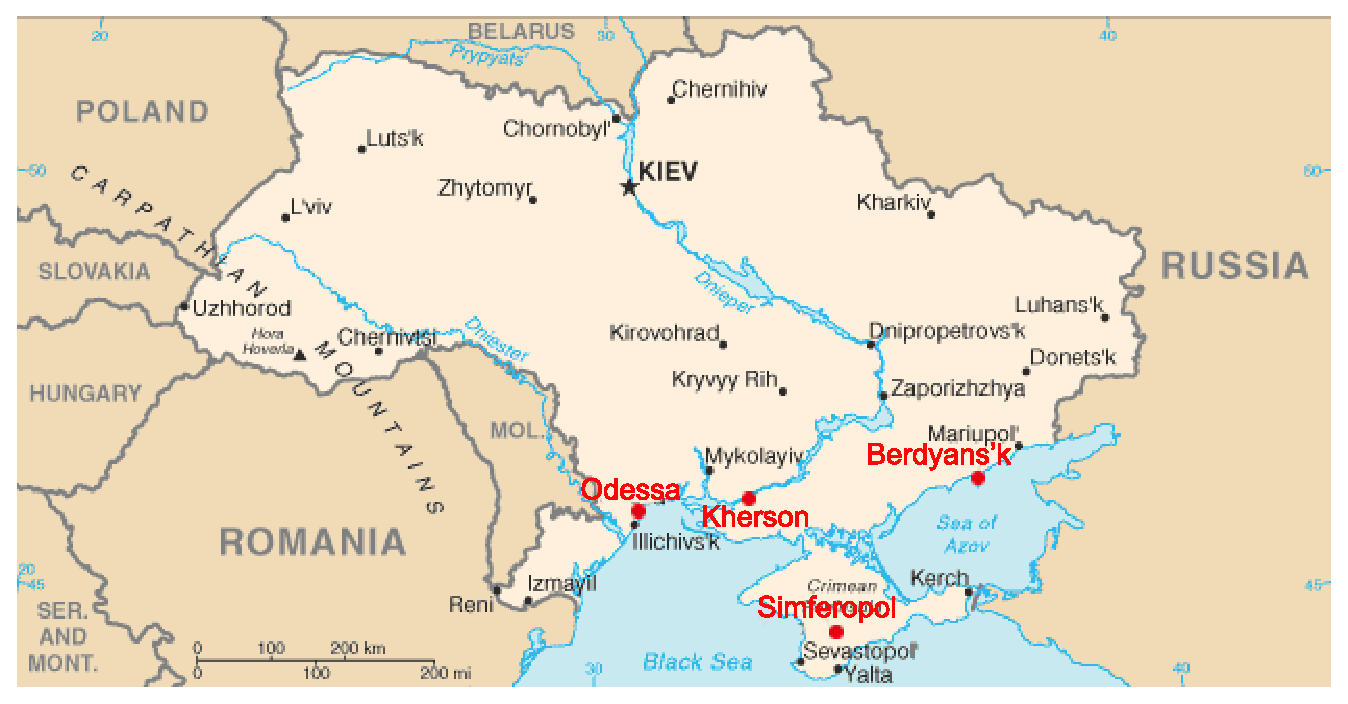
\includegraphics[width=12cm]{./picture/location.eps}\\
  \caption{4 potential locations of desalination plants}\label{location}
\end{figure}
In order to determine the location, we apply Analytic Hierarchy Process(AHP)\cite{Qiyuan}. AHP is a structured technique for organizing and analyzing complex decisions, based on mathematics and psychology. It has particular application in group decision making \cite{Qiyuan}, and is used around the world in a wide variety of decision situations.

We establish our AHP hierarchy shown as figure \ref{AHP}. To obtain the pairwise comparison matrix, we need to compare the influence of $C_1$,$C_2$,...,$C_n$ to the upper level. We follow the comparison scales proposed by Saaty, namely, to use 1-9 to depict the relative influence. Detailed information is shown in Table \ref{scale}.
\begin{figure}[!htbp]
  \centering
  % Requires \usepackage{graphicx}
  \includegraphics[width=14cm]{./picture/AHP.eps}\\
  \caption{AHP hierarchy}\label{AHP}
\end{figure}

\begin{table}[!htbp]
\centering\caption{1-9 scale$a_{ij}$ definition}\label{scale}
\begin{tabular}[ht]{cl}
   \hline
  Scale & Definition\\
   \hline
  1 & $C_i$ and $C_j$ have identical influence\\
  3 & $C_i$ has a little bigger influence than $C_j$ \\
  5 & $C_i$ has greater influence than $C_j$\\
  7 & $C_i$ has an evidently greater influence than $C_j$ \\
  9 & $C_i$ has a dominant influence compared to $C_j$ \\
  2,4,6,8 & the influence of $C_i$ over $C_j$ is between the stated scale \\
  1,1/2,...1/9 & the influence of $C_i$ over $C_j$ is the opposite number of stated scale \\
    \hline
\end{tabular}
\end{table}

Considering the status quo, we define pairwise matrix $A$.
\begin{equation}
A=\left( {\begin{array}{cccc}
    1 & 3 & \dfrac{1}{3} & 2 \\[2ex]
    \dfrac{1}{3} & 1 & \dfrac{1}{9} & 1 \\[2ex]
    3 & 9 & 1 & 6 \\
    \dfrac{1}{2} & 1 & \dfrac{1}{5} & 1 \\[2ex]
  \end{array}}
\right)
\end{equation}

Again, we adopt consistency check approach designed by Saaty, namely \textbf{coincidence indicator}
\begin{equation}
\textit{CI}=\dfrac{\lambda-n}{n-1}\label{CI}
\end{equation}
We can conclude that $A$ is a consistent matrix if \textit{CI}=0; the greater \textit{CI} is, the more likely $A$ to be inconsistent. For the purpose of evaluating the tolerance of inconsistency, we also need to find another criterium to judge \textit{CI}. Saaty introduced \textbf{random indicator}. The process to calculate is to randomly construct matrix $A^\prime$, and then calculate \textit{CI}. Finally the mean value of these \textit{CI} is random indicator. The \textit{RI} table is shown as Table \ref{RI}.
\begin{table}[!htbp]\label{RI}
\centering\caption{\textit{RI} values versus n}
\begin{tabular}{c|ccccccccccc}
  \hline
  % after \\: \hline or \cline{col1-col2} \cline{col3-col4} ...
  n & 1 & 2 & 3 & 4 & 5 & 6 & 7 & 8 & 9 & 10 & 11 \\
  \hline
  \textit{RI} & 0 & 0 & 0.58 & 0.90 & 1.12 & 1.24 & 1.32 & 1.41 & 1.45 & 1.49 & 1.51 \\
  \hline
\end{tabular}
\end{table}

It is clearly seen that $\mbox{\textit{RI}}=0$ when $n=1,2$. This is owing to rank 1 or 2 matrix is always consistent. As for $n\geq 3$, the \textbf{coincidence ratio} is defined as
\begin{equation}\label{CR}
\mbox{\textit{CR}}=\dfrac{\mbox{\textit{CI}}}{\mbox{\textit{RI}}}
\end{equation}
If $\mbox{\textit{CR}}<0.1$, we say it passes consistency check and this matrix can be applied.

According to our matrix, we calculate the eigen value and eigen vector by Matlab:
\begin{equation}
\lambda=4.0752
\end{equation}
\begin{equation}
\textbf{w}=(0.2061,0.0768,0.6184,0.0987)^\prime
\end{equation}\label{vector1}

Applying equation \ref{CI}, $\mbox{\textit{CI}}= \dfrac{0.0752}{3}=0.0251$. We can find \textit{RI}=0.9 from Table \ref{RI}. Hence, follow equation \ref{CR} we get $\mbox{\textit{CR}}=\dfrac{0.0251}{0.9}=0.0279<0.1$. It passes the consistency check.

Next thing, determine the priority factors. In this cite selection issue, we have already got the ratio vector from criteria level to goal level. We need the factors from alternatives level to criteria level. Based on geography of Ukraine, we determine the following matrixes.
\begin{equation}
B_1=\left(\begin{array}{cccc}
        1 & \dfrac{1}{2} & 3 & 1 \\[2ex]
        2 & 1 & 6 & 2 \\
        \dfrac{1}{3} & \dfrac{1}{6} & 1 & \dfrac{1}{3} \\[2ex]
        1 & \dfrac{1}{2} & 3 & 1
        \end{array}\right),
B_2=\left(
      \begin{array}{cccc}
        1 & 1 & 3 & 2 \\
        1 & 1 & 2 & 1 \\
        \dfrac{1}{3} & \dfrac{1}{2} & 1 & \dfrac{1}{2} \\[2ex]
        1 & 1 & 2 & 1 \\
      \end{array}
    \right),
\end{equation}
\begin{equation}
B_3=\left(
      \begin{array}{cccc}
        1 & 1 & 2 & 2 \\
        1 & 1 & 2 & 1 \\
        \dfrac{1}{2} & \dfrac{1}{2} & 1 & 1 \\[2ex]
        \dfrac{1}{2} & \dfrac{1}{2} & 1 & 1 \\
      \end{array}
    \right),
B_4=\left(
      \begin{array}{cccc}
        1 & 2 & 3 & 3 \\
        \dfrac{1}{2} & 1 & 2 & 2 \\
        \dfrac{1}{3} & \dfrac{1}{2} & 1 & 1 \\[2ex]
        \dfrac{1}{3} & \dfrac{1}{2} & 1 & 1 \\
      \end{array}
    \right)
\end{equation}
where $b_{ij}$ in $B_k(k=1,2,3,4)$ relates to the priority scale between $A_i$ and $A_j$ considering criterium $C_k$. Again, we calculate the ratio vectors and eigen values shown in Table \ref{vector2}.
\begin{table}[!htbp]
\centering\caption{Alternative level calculation results}
\begin{tabular}{c|cccc}
  \hline
  % after \\: \hline or \cline{col1-col2} \cline{col3-col4} ...
  k & 1 & 2 & 3 & 4  \\
  \hline
  & 0.2308 & 0.3541 & 0.3483 & 0.4554  \\
  $w_k$ & 0.4615 & 0.2639 & 0.3033 & 0.2628  \\
   & 0.0769 & 0.1180 & 0.1742 & 0.1409  \\
   & 0.2308 & 0.2639 & 0.1742 & 0.1409  \\
  \hline
  $\lambda_k$ & 4 & 4.2361 & 3.8708 & 4.0104  \\
  \hline
  $\mbox{\textit{CI}}_k$ &0&0.0787&0.0431&0.0035 \\
  \hline
\end{tabular}\label{vector2}
\end{table}

What needs to be clarified is that all the \textit{CI}s have passed the check.
Lastly, we combine all of the priority factors to achieve the final priority index, which is simply the product of two priority vectors: \eqref{vector1} and Table \ref{vector2}. By multiplying these two vectors we get
\begin{equation}
\mbox{\textbf{$w_f$}}=[0.3351,0.3289,0.1465,0.1895]^\prime
\end{equation}
We can tell from the results that we pick Odessa to be the best cite to build desalination plants.

\subsection{Intervention Advantages and Weaknesses}
Like any model,the one present above has its strengths and weaknesses. Some of the major points are presented below.
\subsubsection{Advantages}
\begin{itemize}
\item \textbf{Alleviating the water stress in the south}\\
One of the most significant strengths is to drastically alleviate the water stress issue by providing the country more fresh water from Black sea. Since the South is the most serious place in Ukraine, and by establishing a desalination plant here in a coastal city, people can utilize water from the ocean, taking advantage of technology to transform salty water to edible clean water. This method can increase total available water resources.
\item \textbf{Renewable}\\
The raw materials of desalination plants are mainly seawater which is renewable. This coincides with the idea of sustainable development.
\item \textbf{Providing more employment opportunities}\\
The plan to establish desalination plants can produce many employment opportunities. Workers, constructors, technical workers, supervisors, etc. are abundantly needed in the region. Therefore, it can also alleviate the social instability caused by high unemployment rate.
\end{itemize}

\subsubsection{Weaknesses}
\begin{itemize}
\item \textbf{Gigantic initial investments}\\
Establishing desalination plants requires both advanced technology and gigantic capital.
\item \textbf{Rising price of water}\\
Compared to the normal water resources, water from desalination needs more efforts and therefore, has higher prices. To maintain the operation of plants, the price of water will rise which may lead to indignation of inhabitants.
\item \textbf{Possible negative effects on the ocean}\\
Desalination can have some side effects on the ocean ecological system. Those substances in the seawater will not disappear and since people only take water from the ocean, it may cause the imbalance of ion density.
\end{itemize}

%===============================模型结果============================================
\section{Intervention Effectiveness}
Just as mentioned above, desalination is an effective way to solve the water scarcity. According to survey conducted by International Desalination Association (IDA)\cite{EL}, the world's desalination volume is increasing rapidly by 10\%-30\%. Up till now there are more than 130 countries are using this technology to get water. Interestingly, more than half of the desalination is in Middle East. The world's pie chart is shown in Figure \ref{piechart} \cite{Junhong}.
\begin{figure}[!htbp]
  \centering
  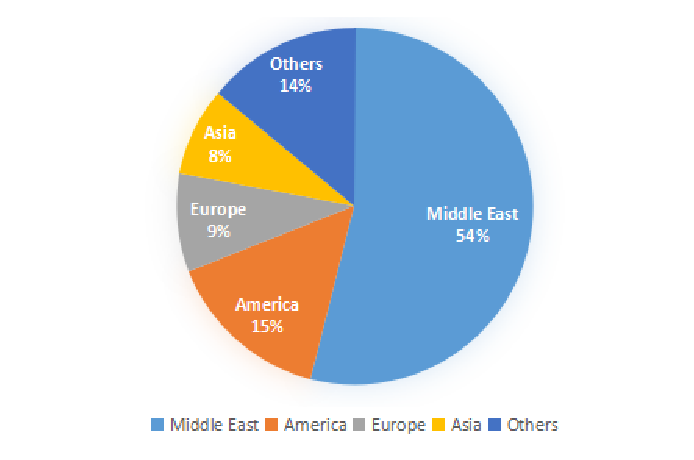
\includegraphics[width=9cm]{./picture/piechart.eps}\\
  \caption{World's desalination distribution}\label{piechart}
\end{figure}

Considering the similarities between China and Ukraine, we decide to transplant China's development goals to desalination, shown as Table \ref{goals}.
\begin{table}[!htbp]
\centering\caption{Desalination goals in Ukraine in 15 years}
\begin{tabular}{cc|cccc}
  \hline
  % after \\: \hline or \cline{col1-col2} \cline{col3-col4} ...
  Year &  & 2016 & 2020 & 2025 & 2030 \\
    \hline
  Desalination & $\times 10^4 m^3/d$ & 3 & 100 & 300 & 800 \\
  Scale & $\times 10^4 m^3/d$ & 0.5 & 10 & 20-50 & 50-80 \\
  Tech-independency ratio & \% & 10 & 60 & 90 & 100 \\
  Investment & $\times 10^8 USD$ & 10 & 15 & 35 & 90 \\
  \hline
\end{tabular}\label{goals}
\end{table}

By this rough goal, we get possible curves of desalination shown in Figure \ref{fitting}. The line of best-fit is
\begin{equation}
f(x)=0.3036x^3 -1838x^2 + 3.71\times10^6x -2.496\times10^9
\end{equation}
The fitting residual is $6.457\times10^{-11}$, which indicates a great fitting (Appendix J).
\begin{figure}[!htbp]
  \centering
  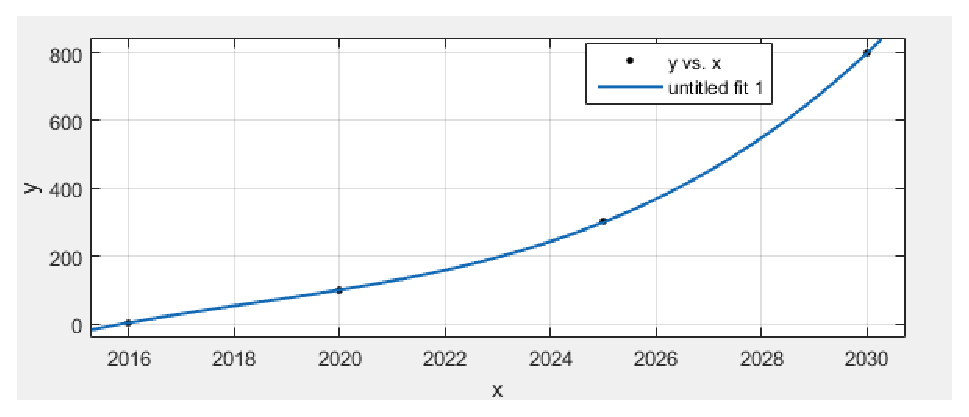
\includegraphics[width=8cm]{./picture/fitting.eps}\\
  \caption{Fitting curve of desalination in Ukraine in 15 years}\label{fitting}
\end{figure}

After doing some arithmetic calculations, we finally get that form 2016 to 2030, Ukraine can produce 115.177 billion $m^3$ clean water from desalination (Appendix K). Thus, the mean of these 15 years is 7.678 billion $m^3$. From the above Table \ref{predicted2}, we know the mean of annual withdrawal water is 15.659 billion $m^3$. If we take the quotient of these two values, we get $\dfrac{7.678}{15.659}=49.03\%$. Thus, from an average scale, we notice that desalination plants can effectively provide clean water to Ukraine.


%========================模型的实效分析(适应性说明)=============================
\section{Conclusions}
Based on our model results, we find that Ukraine will experience more severe water stress in next 15 years. For one thing, geologically speaking, Ukraine is a country that suffers from renewable water resources. Water resources per capita in Ukraine less than the international water shortage warning line standard; temporal and spatial distribution of water resources in Ukraine is quite uneven; and Ukraine's water dependency ratio is very high. For another, Ukraine's social factors account for this issue as well. The daily water consumption per capita in Ukraine as well as the large amount of industrial withdrawal has made this country even more vulnerable. In a nutshell, this water use pattern is leading Ukraine to a rather serious situation.

For the purpose of addressing this issue, we propose to build a desalination plant in Odessa, which is located in southern coastal area. This method can effectively alleviate the water stress in the region. Besides, it coincides with the idea of sustainable development. However, it may need large amount of investments and might intrigue the rise of water price.

%================================总体评价==============================
\section{Evaluation of Model}
Like any other model, the one presented above has its strengths and weaknesses. Some of the major points are presented below.
\subsection{Strengths}
\begin{itemize}
\item \textbf{Broad application}\\
This model can be used for many countries, not only for Ukraine, as long as we have enough data of other countries. Therefore, this model can be transplanted to adapt to many situations.
\item \textbf{Comprehensive and Systematic}\\
This model can contain various kinds of data to complete prediction, and by taking as many as data into consideration as possible, the prediction will be more comprehensive and systematic, more likely to be achieve accurate estimation.
\item \textbf{Excellent generalization ability}\\
The core of this model is Back Propagation. BP ensures excellent generalization ability (the ability to adapt to new training samples). The model can respond correctly in spite of some noisy inputs.
\end{itemize}
\subsection{Weaknesses}
\begin{itemize}
\item \textbf{Inaccuracy for long-term prediction}\\
Just like any prediction model, our model can't ensure its reliability for long-term prediction either. This is because of the bare fact that the model can no longer rectify its error for the lack of real values.
\item \textbf{Fluctuation on results}\\
TGB model's output can vary from time to time, yet within an acceptable range. This fluctuation may be magnified with the length of prediction period. That is to say, this model cannot give high-precision accurate quantitative values.
\end{itemize}

\begin{thebibliography}{99}
%\addcontentsline{toc}{section}{References}
\bibitem{1}Shashi Sathyanarayana. "A Gentle Introduction to Backpropagation", 2014: 4-13.
\bibitem{2}Wang, Shuo, et al. "Multi-scale analysis of the water resources carrying capacity of the Liaohe Basin based on ecological footprints", Journal of Cleaner Production, 2013: 158-166.
\bibitem{Wengao Lou}Wengao Lou, Suiqing Liu. "On Assessment of Sustainable Development Level of Regional Water Rsource Using Artificial Neural Networks", System Sciences and Comprehensive Studies in Agriculture, 2003: 114-119.
\bibitem{Qingwen}Qingwen Min, et al. "Fuzzy-based Evaluation of Water Resources Carrying Capacity and its Application", 2004: 14-16.
\bibitem{Liyu Han}Liyu Han. "Development and utilization of water resources in Ukraine", China Academic Journal Electronic Publishing House, 2009: 61-66.
\bibitem{Lang Xu}Lang Xu. "Study on the water resources carrying capacity in Jiangsu Province based on principal component analysis", Resources and Environment in the Yangtze Basin, 2011: 1468-1474.
\bibitem{Xiangui}Xiangui Xue, Lu Li. "Evaluation of water resources carrying capacity in Guizhou based on BP neural network", Fujian Computer, 2015: 8-9.
\bibitem{Shitang Ke}Shitang Ke, et al. "Prediction on Wind Effects of Large Cooling Towers Based on Grey-Neural Network Joint Model", Journal of Nanjing University of Aeronautics and Astronautics, 2014: 652-658.
\bibitem{Jianyong Liu}Jianyong Liu, et al. "Forecasting model for development cost of equipment based on artificial neural network and grey Verhulst algorithm", Journal of PLA University of Science and Technology, 2008: 335-338.
\bibitem{EL}El-Dessouky H T, et al. "Multi-stage Flashi Desalination", Present and Future Outlook, 1999: 173-190.
\bibitem{Junhong}Junhong Wang, et al. "Development and application of seawater desalination", Industrial Water Treatment, 2008: 6-9.
\bibitem{Qiyuan}Qiyuan Jiang. Mathematical Model(4th Edition).
\bibitem{AQUA}AQUASTAT. Food and Agriculture Organization of the United Nations. FAO Water Resources. http://www.fao.org/nr/water/aquastat/water\_res/index.stm
\bibitem{wri}World Resource Institute. http://www.wri.org/
\bibitem{3}http://www.latexstudio.net/
\bibitem{4}http://www.chinatex.org/
\end{thebibliography}

%====================附录导入程序代码==========================================
\begin{appendices}
    %\renewcommand{\thesection}{\Alph{chapter}.}
  \section{}
\lstinputlisting[language=Matlab]{./code/ann2.m}
  \section{}
\lstinputlisting[language=Matlab]{./code/picture.m}
  \section{}
\lstinputlisting[language=Matlab]{./code/resmean0.m}
  \section{}
\lstinputlisting[language=Matlab]{./code/GM1GM11.m}
  \section{}
\lstinputlisting[language=Matlab]{./code/GM2DGM.m}
  \section{}
\lstinputlisting[language=Matlab]{./code/GM3Verhulst.m}
  \section{}
\lstinputlisting[language=Matlab]{./code/grey.m}
  \section{}
\lstinputlisting[language=Matlab]{./code/resmean.m}
  \section{}
\lstinputlisting[language=Matlab]{./code/s11.m}
  \section{}
\lstinputlisting[language=Matlab]{./code/fitting.m}
  \section{}
\lstinputlisting[language=Matlab]{./code/integral.m}

    \end{appendices}


\end{document}
%%%%%%%%%%%%%%%%%%%%%%%%%%%%%%%%%%%%%%%%%%%%%%%%%%%%%%%%%%%%%%%%%%%
%%%%%%%%%%===========THE END OF PAPER============%%%%%%%%%%%%%%%%%%
%%%%%%%%%%%%%%%%%%%%%%%%%%%%%%%%%%%%%%%%%%%%%%%%%%%%%%%%%%%%%%%%%%%
